\documentclass[12pt]{article}
%\usepackage[utf8]{inputenc}
%\documentclass[UTF8]{ctexart}
%\usepackage[UTF8, heading = false, scheme = plain]{ctex}
\usepackage{geometry}
%geometry{a4paper,scale=0.9}
\geometry{a4paper,left=1cm,right=1cm,top=1cm,bottom=2cm}
\usepackage{amsfonts}
\usepackage{color}
\usepackage{url}
%\usepackage{biblatex}
\usepackage{amsmath}
\usepackage{amssymb}
\usepackage{latexsym}
\usepackage{cite}
%\addbibresource{ref.bib}
%\bibliography{ref.bib}
\usepackage{caption}
\usepackage{graphicx, subfig}
\usepackage{float}
%\usepackage[fontset=ubuntu]{ctex}
%\usepackage{fontspec}
\usepackage{xeCJK}
%\usepackage[colorlinks,
%anchorcolor=black,
%citecolor=black]{hyperref}
%\setmainfont{SimSun}
\usepackage[section]{placeins}
\usepackage{enumitem}
\usepackage{framed}
\usepackage[framemethod=TikZ]{mdframed}
\usepackage{indentfirst}
\usepackage{setspace}%使用间距宏包
\linespread{1.5}

\title{因果推断概述\cite{Causal_Inference_Simply_Introduction}\cite{Talk_About_Causal_Inference_Part_1}\cite{AAAI_2020_Tutorial_Representation_Learning_for_Causal_Inference}}
\author{leolinuxer}
%\date{June 2020}

\begin{document}
%\setlength{\parindent}{0pt}
\maketitle
\tableofcontents

\section{因果性与相关性}
\subsection{因果性与相关性的比较}
事件/变量之间的关系,最主要的有\textbf{相关性}和\textbf{因果性}。
\begin{itemize}
\setlength{\itemsep}{0pt}
\setlength{\parsep}{0pt}
\setlength{\parskip}{0pt}
    \item 相关性是指在观测到的数据分布中,$X$与$Y$相关,如果我们观测到$X$的分布,就可以推断出$Y$的分布;
    \item 因果性是指在操作/改变$X$后,$Y$随着这种操作/改变也变化,则说明$X$是$Y$的\textbf{因cause};
\end{itemize}

在常用的机器学习算法中,关注的是特征之间的相关性,而无法去识别特征之间的因果性,而很多时候在做决策与判断的时候,我们需要的是因果性。

举个例子,我们会发现在学校中,近视的同学成绩更好。近视和成绩好之间有强相关性,但显然近视不是成绩好的原因。而我们想要提升学生成绩,自然需要找到因,否则就会通过给学生戴眼镜的方式来提高成绩。这个例子是很明显地可以区分出相关与因果的,但是也有很多难以区分的,如经常喝葡萄酒的人寿命更长,是因为葡萄酒确实能延长寿命,还是因为能经常喝的人通常更富有,享有更好的医疗条件。再比如:
\begin{itemize}
\setlength{\itemsep}{0pt}
\setlength{\parsep}{0pt}
\setlength{\parskip}{0pt}
    \item 在 feeds 流里刷到一个新推荐策略的内容的用户留存更高,他们的高留存是因为这个推荐策略导致的吗,这个策略究竟对留存的提升有多大效果?
;
    \item 上周投放了某游戏广告的用户登录率更高,他们的高登录率有多大程度是由广告带来的,有多大程度是由于他们本身就是高潜力用户?
\end{itemize}


\subsection{识别因果的必要性}
有些时候,我们通过统计学方法或者机器学习算法得到的特征之间的相关性,就足以为我们的验证、决策提供指导,比如,我们通过数据发现,用户曝光的图片越多,留存越高,我们不需要知道这之间是否有复杂的因果关系,只需要通过简单的ABtest来检验更多的曝光是否有效果即可。

在这些例子中,本质上,我们都是想要分析一个干预(treatment)对一个结果(outcome)有怎样的影响,想要探究其中的因果效应。大家熟悉的 A/B Test 是回答上面这些问题的黄金方式。但是,A/B Test 也有一定的局限性,例如:
\begin{itemize}
\setlength{\itemsep}{0pt}
\setlength{\parsep}{0pt}
\setlength{\parskip}{0pt}
    \item 药物是否有效、政策是否有效,这种问题无法做 ABtest;
    \item 新的推荐算法是否有效,ABtest成本高(不好的用户体验等);
    \item 需要花一定的时间实现,比较耗费人力;
    \item 需要占用足量的随机流量,并且需要持续一段时间以收集数据;
    \item 当可做 A/B Test 的选择太多时,往往难以全部都进行尝试。
\end{itemize}

因此,面对这种特殊的问题,我们需要\textbf{从已有的数据}中推断出变量间的因果性。

\section{因果推断的相关概念}
\subsection{核心概念}
\textbf{因果关系(Causality)}:如果其他变量不变,当且仅当T的改变会导致Y的改变时,T 与 Y 有因果关系;(T causes Y if and only if changing T leads to a change in Y,while keeping everything else constant. )\cite{Causal_Inference_and_Stable_Learning}

\textbf{因果效应(Causal effect)}:当T导致Y改变时,Y 改变的“幅度”;(Causal effect is defined as the magnitude by which Y is changed by a unit change in T.)

\textbf{结构化因果模型(Structural Causal Model):}A graphical model to describe the causal mechanisms of a system.
\begin{figure}[H]
    \centering
    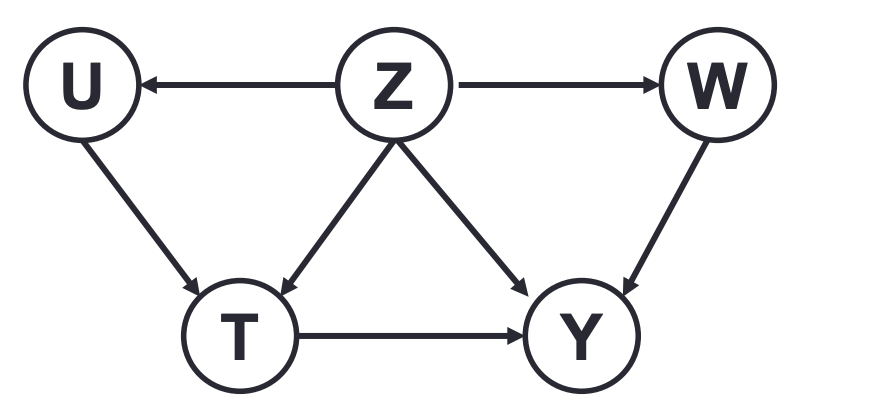
\includegraphics[width=0.5\textwidth]{fig/Causal_Inference_and_Stable_Learning-Causal-Model.png}
\end{figure}

\subsection{相关术语\cite{AAAI_2020_Tutorial_Representation_Learning_for_Causal_Inference}}
\textbf{confounder(混淆因子)}:Variables that affect both treatment assignment and outcome;(既影响试验方案(??),也影响结果的变量)

例如:在药物试验中,年龄就是一个 confounder,原因是:
\begin{itemize}
\setlength{\itemsep}{0pt}
\setlength{\parsep}{0pt}
\setlength{\parskip}{0pt}
    \item 年龄会影响药物的治愈率(Age would affect the recovery rate);
    \item 年龄会影响实验方案(??)的选择(Age would also affect the treatment choice);
\end{itemize}

从下图可以看出来,年龄变量会导致辛普森悖论。
\begin{figure}[H]
    \centering
    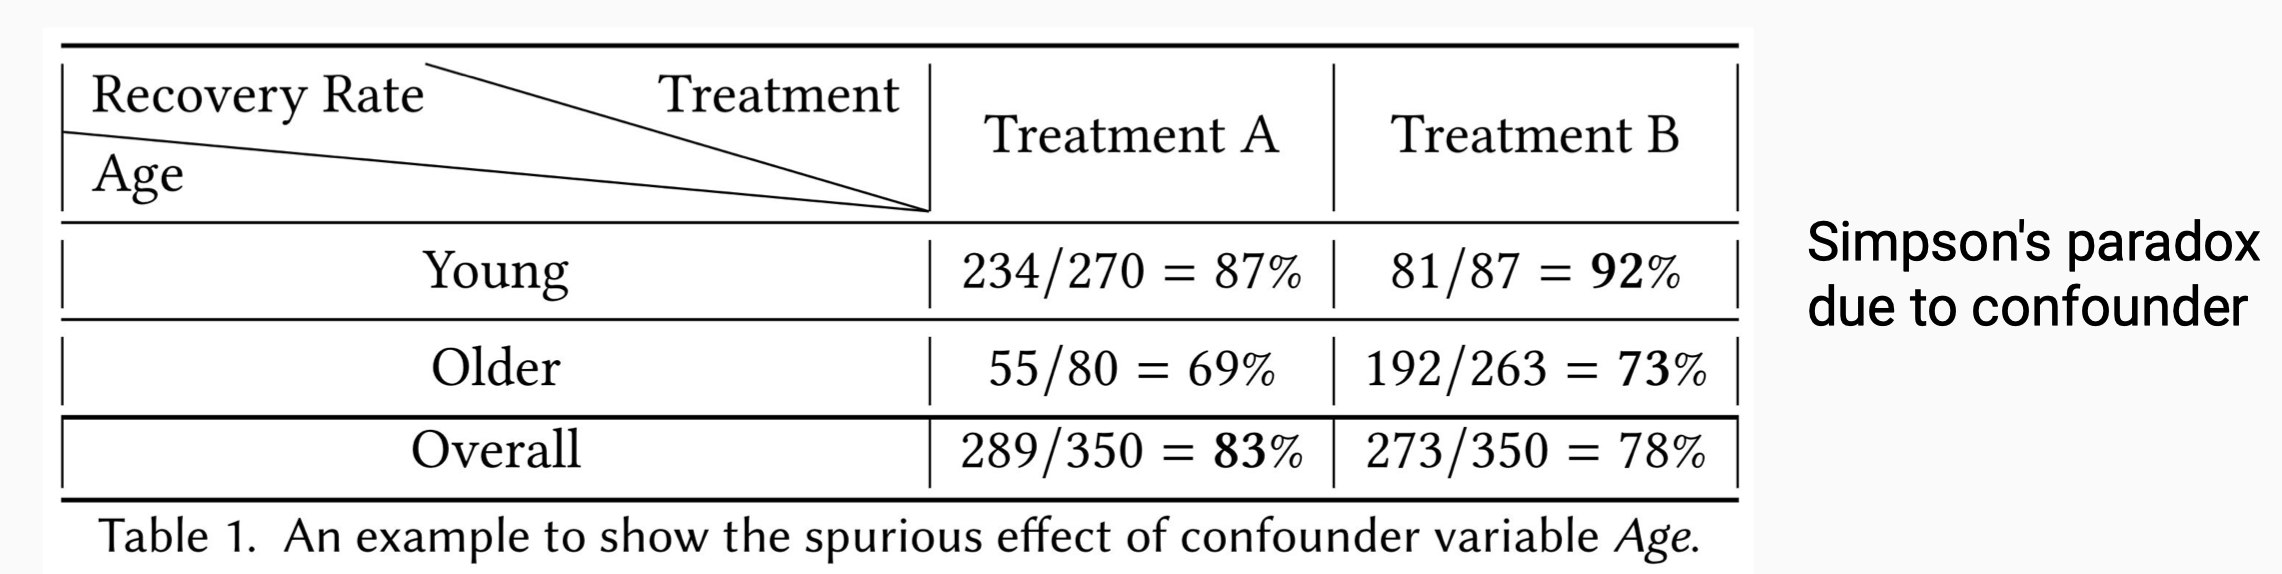
\includegraphics[width=1\textwidth]{fig/CasualInference-Confounder-Example-In-Medicine.png}
\end{figure}

\textbf{Selection Bias}:The distribution of the observed group is not representative to the group we are interested in;

Confounder variables affect units' treatment choices, which leads to the
selection bias; Selection bias makes counterfactual outcome estimation more difficult.

\subsection{相关符号定义}
\begin{itemize}
\setlength{\itemsep}{0pt}
\setlength{\parsep}{0pt}
\setlength{\parskip}{0pt}
    \item \textbf{干预 (treatment) $T$}:一般我们考虑二值干预,用 $T_i \in \{0,1\}$ 来指示用户是否受到了某种干预,例如是否被投放了某广告、是否被灰度了某功能。在 A/B Test 中,实验组的用户都受到了某种处理,他们都有 $T_i=1$。

    \item \textbf{潜在结果(potential outcome)$\{Y_{i0}, Y_{i1}\}$}:对每个用户 $i$,他们对于是否受到干预分别有两个潜在结果 $Y_{i0}$ 和 $Y_{i1}$。例如,$Y_{i0}$ 和 $Y_{i1}$ 分别表示假如一个用户没有被投放游戏广告和被投放时是否会登录游戏。
    
    \item \textbf{观察结果(observed outcome)$Y$}:当一个用户没有受到干预时($T=0$),我们将会观察到 $Y=Y_{i0}$,当一个用户受到干预时我们将会观察到 $Y=Y_{i1}$。
    
    \item \textbf{反事实结果(Counterfactual Outcome)}:假设一个用户没有收到干预的潜在结果;反事实结果无法被观察到;
\end{itemize}


\subsection{因果效应的度量方式}
在因果分析中,我们通常比较关心以下两种 “因果效应”。为了符号简洁,接下来不再特意标注出代表用户的下标 :
\begin{itemize}
\setlength{\itemsep}{0pt}
\setlength{\parsep}{0pt}
\setlength{\parskip}{0pt}
    \item \textbf{平均因果效应 (Average Treatment Effect,简称 ATE)}: $ATE=E[Y_1 - Y_0]$。$ATE$ 为干预对所有人的平均因果效应。

    \item \textbf{干预组的平均因果效应(Average Treatment Effect on the Treated,简称 ATT)}:$ATE=E[Y_1 - Y_0|T = 1]$。$ATT$ 为干预对受到干预的人的平均因果效应。
\end{itemize}

以游戏广告投放为例,假如我们可以同时观测到两个潜在结果(\textbf{尽管这是不可能的}),我们可以算出 
\begin{figure}[H]
    \centering
    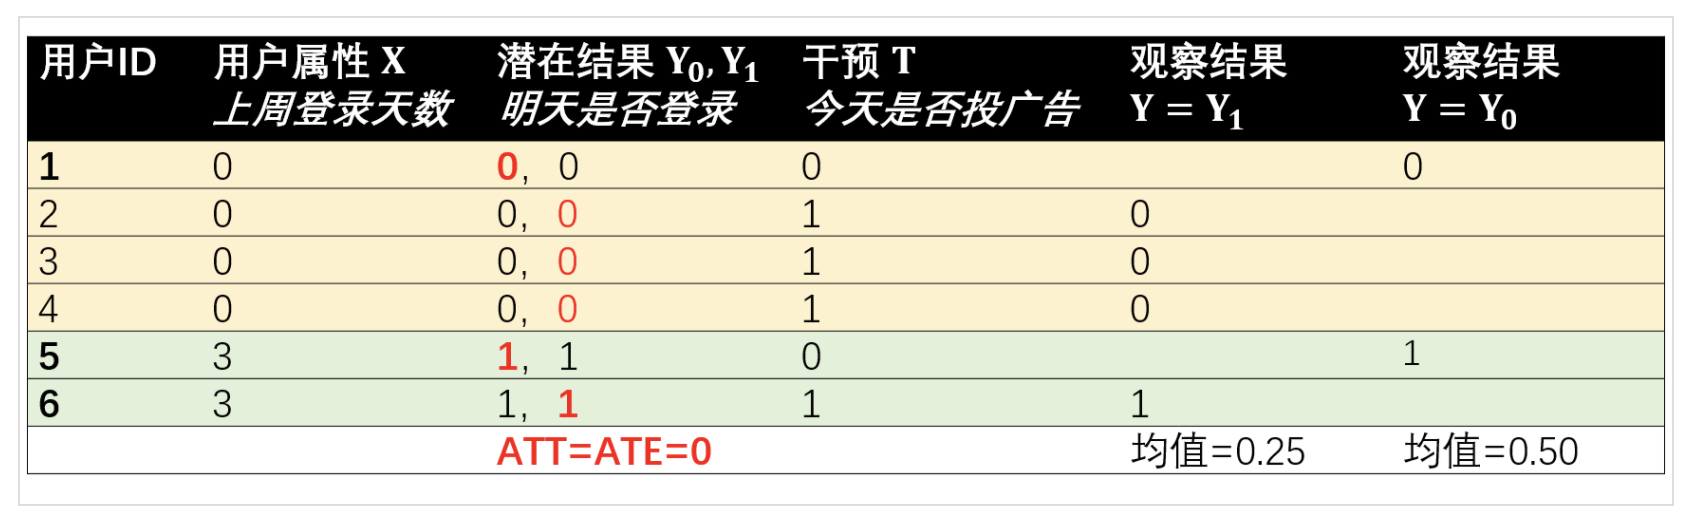
\includegraphics[width=1\textwidth]{fig/CasualInference-Game-Ad-1.png}
\end{figure}

当我们尝试直接从观察结果$Y$  统计 $ATE$ 或者 $ATT$ 时,我们就会遇到一个问题:对于每一个用户,我们并不能同时观测到两个潜在结果。这个问题是因果推断的一个核心问题、核心难点。

\subsection{因果推断的核心思想}
\begin{mdframed}[
linecolor=black!40,outerlinewidth=1pt,roundcorner=.5em,innertopmargin=1ex,innerbottommargin=.5\baselineskip,innerrightmargin=1em,innerleftmargin=1em,backgroundcolor=gray!5,
%backgroundcolor=blue!10,%userdefinedwidth=1\textwidth,%shadow=true,%shadowsize=6,%shadowcolor=black!20,%frametitle={The \textit{two-step} model of XMCD:},%frametitlebackgroundcolor=cyan!40,%frametitlerulewidth=10pt
]
\textbf{因果推断的核心思想在于\textcolor{red}{反事实推理counterfactual reasoning},即在我们观测到$X$和$Y$的情况下,推理如果当时没有做$X$,$Y'$是什么。}
\end{mdframed}

因果推断的目的是要判断因果性,即计算\textbf{因果效应}(有无$X$的情况下$Y$值的变化量)。在进行反事实推理后,可得出\textbf{因果效应}$e = |Y - Y'|$,进而判断因果性。

实际上,对于一个对象,我们永远只能观察到$Y$和$Y'$的其中一个,因果推断所做的就是从已有数据中估计因果效应,所以我认为因果推断的本质是对因果效应的估计。

A/B Test 提供了解决这个核心问题的完美方案,让我们通过简单的公式看看为什么。在做 A/B Test 时,我们一般直接统计实验组和对照组的指标差异。
根据 $ATT$ 的定义,我们可以得到如下公式推导
$$
ATT = E[Y_1 - Y_0 | T=1] = (E[Y_1|T=1] - E[Y_0|T=0]) - (E[Y_0|T=1] - E[Y_0|T=0]) = \hat{ATT} + bias
$$

其中,$\hat{ATT}$定义为:
$$
\hat{ATT} = E[Y_1 | T = 1] - E[Y_0|T=0]
$$

这里的 bias,根据定义来看,是实验组和对照组的潜在结果 $Y_0$ 的差异。在 A/B Test 中,我们假设实验组和对照组是随机划分的,因此 bias 为 0。因此,根据 A/B Test 计算的 $\hat{ATT}$ 就是 $ATT$ 的无偏估计。即$\hat{ATT}$就是我们的估算方式。

在日常工作中,并非所有数据分析都有 A/B Test 撑腰。我们往往需要通过观察历史数据完成分析,这类分析称为 “观察性研究”。在观察性研究中,失去了 “随机流量” 的撑腰,现实就没有那么美好了。这时,如果我们直接比较两组用户指标上的差异得到 $\hat{ATT}$,它和真实的 $ATT$ 之间是存在一个非零的 bias 的,我们无法根据  $\hat{ATT}$ 下一个科学可靠的结论。 例如,在之前使用的广告投放的例子中,假设我们直接比较 $T=1$ 和 $T=0$ 两组用户的观测结果 $Y$的差异,会造成投放广告造成登录率从 50\% 下跌到 25\% 的错觉,这并不是真实的 $ATE$ 和 $ATT$。


\section{因果效应可识别性的前提假设}
在观察性研究中,借助什么样的数据可以推出可靠的因果效应($ATE$ 或 $ATT$)呢?具体来说,假如我们对每个用户有一系列干预前的指标(pre-treatment variables) $X$、有干预 $T$、有观察结果 $Y$,我们能不能推断出 $T$ 对 $Y$ 的因果效应?
这个问题就是因果推断的可识别性(identifiability)问题。可识别性依赖于几个假设,这些假设通常被称为 causal assumption。下面我们一个一个来看看。

\subsection{Stable Unit Treatment Value Assumption (SUTVA)}
SUTVA 假设用户之间是相互独立的,无互相干扰。SUTVA 保证个体的潜在结果只和他自己有关、最终观察到的结果也只和他自己有关。值得注意的是,社交网络上的实验理论上都很难完完全全保证 SUTVA,但是对于大部分社交属性不强的实验,一般还是假设 SUTVA 基本成立。

\subsection{Ignorability}
Ignorability 假设对于 pre-treatment 变量 $X$ 一样的人群,是否接受处理和潜在结果相互独立:$Y_0, Y_1 \bot T|X$。$\bot$ 表示独立性。

这个假设比较难以理解,我们套用之前举的广告投放的例子看看。在这个例子中,我们倾向于给历史登录天数少的用户投放广告,$X$ 和 $T$ 是负相关的。同时,历史登录天数越多,未来登录率也越高,即 $X$ 和潜在结果 $Y_0$ 和 $Y_1$ 都是正相关的。在这份数据里,$(Y_0, Y_1)$ 和 $T$ 并不独立。但是,对于 $X$ 取值一样的用户,是否看到广告可以看做是随机的,ignorability 成立。

Ignorability 这个假设还有很多其它的名字,例如 no unmeasured confounders assumption 和 Conditional Independence Assumption (CIA)。

\subsection{Consistency}
Consistency 假设潜在结果和观察到的结果是一致的,即当 $T = t$时 $Y = Y_t$。这个假设一般可以认为是成立的。

\subsection{Positivity}
Positivity 假设要求 treatment assignment 有一定随机性,要求对于$X$ 的所有取值都有 $ 0 < Pr[T=1|X=x] < 1$。如果这个假设不成立,我们是无法下结论的。例如当一部分用户不可能被投放广告时,我们无法通过历史数据分析广告对他们的效果。当 positivity 假设不成立时,我们往往需要考虑去除一些特殊用户群。

Positivity 这个假设也有些其它的名字,常见的有 common support 和 overlap。

A/B Test 满足上面的每一个假设。在观察性研究中,SUTVA、ignorability 和 consistency 这三个假设都是无法验证的(untestable)。有时我们可以通过一些经验或是数据判断出这些假设明显不成立,但是我们没有办法可以证明这些假设成立。

\section{一些因果推断的方法}
\subsection{随机实验Randomization}
\subsubsection{A/B Test}
以推荐算法为例,判断推荐算法是否有效,ABTest通过将用户随机分为两组,分别应用不同的算法,通过判断两组用户点击率的差异来估计因果效应。通过随机分组,排除了混淆变量的影响。

A/B Test实际上是判断因果性的很有效的方法,但有时候成本过高无法采用,如这里的推荐算法——
\begin{itemize}
\setlength{\itemsep}{0pt}
\setlength{\parsep}{0pt}
\setlength{\parskip}{0pt}
    \item 可能新的推荐算法太差导致用户流失;
    \item 如果有很多新的算法要测试,A/B Test效率较低;
\end{itemize}

\subsubsection{多臂老虎机 Multi-armed bandits}
针对上述问题,另一种随机实验方法是强化学习中的多臂老虎机,实际上是\textbf{对explore和exploit的平衡}。
\begin{itemize}
\setlength{\itemsep}{0pt}
\setlength{\parsep}{0pt}
\setlength{\parskip}{0pt}
    \item explore,随机选择一个动作,在上面的问题中是随机选择一个算法;
    \item exploit,选择收益最高的动作,在上面的问题中是选择当前效果最好的算法;
\end{itemize}

通过某种规则(e-greedy等)重复上述过程,优点是可以同时测试多种算法,并且每个用户都能使用到最好的算法,减少流失可能性。缺点是效果难以评估,也很难让用户按照我们的想法行动。

\subsection{自然实验Natural Experiments}
理想的实验需要:\textbf{随机分配(分组)、人为干预(施加不同的treatment)、结果比较}。

自然实验实际上是一种\textbf{观察性研究},满足上述三个条件中的两个,是指不加干预地、实验对象\textbf{“自然”}地分为若干组,对实验对象的结果进行观察比较。

显然自然实验法的关键在于,实验对象是否能“自然”/随机地分组。比如,将是否民主将国家分为两组,探究制度与国家对外战争的关系。但是在这里,是否民主不是随机的分给各个国家,所以无法满足自然实验所需的随机分配原则。

\subsubsection{断点回归Regression discontinuity}
断点回归是自然实验中的一种观察方法,简单理解就是在回归过程中,观察在临界点处是否出现断层/断点。

举一个简单的例子,假设现在有一个产品,收集500个金币后就可以得到一个勋章,现在要判断有无勋章对用户在线时长的影响。断点回归法观察金币在500附近的用户,如497到502,观察【接近500但小于500(无勋章)】与【接近500但大于500(有勋章)】的用户在线时长是否有显著区别,若有,说明有勋章很可能会增加用户的在线时长。

\subsubsection{工具变量Instrumental Variables}
对于要判断因果关系的两个变量间,如果存在其他混淆变量,在计量经济学中采用工具变量的方法解决。

以下述关系为例,要判断对APP1的访问,是否会导致对APP2的点击。实际上由于APP1和APP2之间的需求关系,误差项与解释变量相关,即计量经济学中的内生性。
\begin{figure}[H]
    \centering
    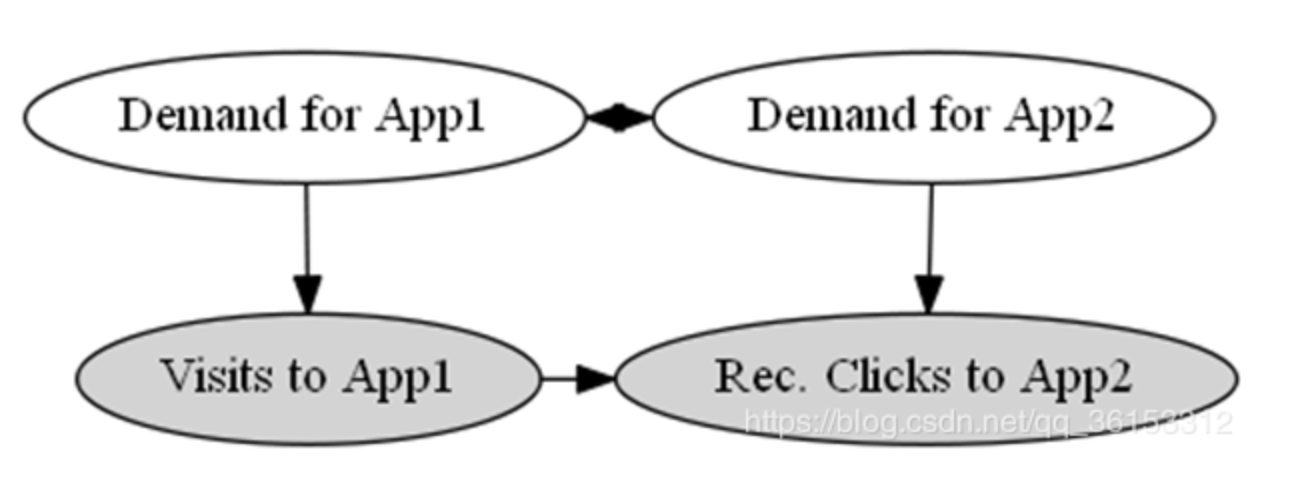
\includegraphics[width=0.8\textwidth]{fig/CasualInference-APP-User-Example.png}
\end{figure}

\textbf{引入工具变量的目的是为了让误差项与解释变量不相关}。具体地,通过找到一个变量,满足与解释变量相关且与误差项无关,那在引入这一变量之后,解释变量变化的部分就与误差项无关。

同样是上面的例子,假设某一天有个活动,下载APP1的人有奖励,这个活动与解释变量相关,但不会影响到APP2的需求,那根据多出来的APP1访问量与多出来的APP2点击率就不再受到需求关系的影响,就可以判断对APP1的访问,是否会导致对APP2的点击。
\begin{figure}[H]
    \centering
    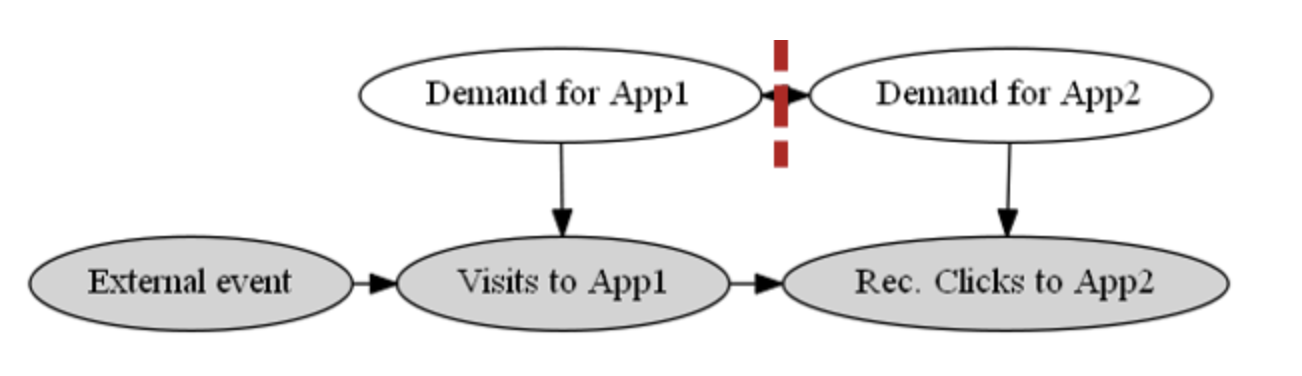
\includegraphics[width=0.8\textwidth]{fig/CasualInference-APP-User-Example2.png}
\end{figure}

\subsection{Conditioning}
\subsubsection{分层Stratification}
分层的核心思想是控制条件变量,一般步骤如下:
\begin{itemize}
\setlength{\itemsep}{0pt}
\setlength{\parsep}{0pt}
\setlength{\parskip}{0pt}
    \item 尽可能完整的绘制出变量之间的因果图
    \item 选择影响要判断因果性的变量的条件变量
    \item 对用户进行分层/分组,满足组内的用户条件变量取值一致(上层的变量将全部不需要再考虑,类似贝叶斯网络中的d分隔)
    \item 比较两组用户的输出,计算因果效应
\end{itemize}
这种方式有点类似要找到相似的用户,当条件变量很多的时候,这种方法很难实现,很难找到很多条件变量都相同的用户,即使找到也会使得分组偏小。

\subsubsection{倾向得分匹配Propensity score matching}
当条件变量很多的时候,可以考虑使用倾向得分匹配。

以推荐算法为例,当条件变量很多的时候,通过逻辑回归等方法对这些变量进行训练,并计算出一个倾向得分,在这里是用户被施加新算法的概率。因此倾向得分匹配的一般步骤如下:
\begin{itemize}
\setlength{\itemsep}{0pt}
\setlength{\parsep}{0pt}
\setlength{\parskip}{0pt}
    \item 尽可能完整的绘制出变量之间的因果图
    \item 选择影响要判断因果性的变量的条件变量
    \item 对用户进行分层/分组,满足组内的用户计算得出的倾向得分接近(上层的变量将全部不需要再考虑,类似贝叶斯网络中的d分隔)
    \item 比较两组用户的输出,计算因果效应
\end{itemize}

\subsection{Matching 方法详解}
假设我们有一份数据,我们判断几个 causal assumption 都是成立的,我们应该如何推断其中的因果效应呢?基于潜在结果模型,一套比较经典的因果效应推断方式是 Matching。Matching 这个方法从名字来看很直观,但是里头还是有一些套路的。

最最基本款的 Matching 是 Exact Matching。假设我们感兴趣的因果效应是 $ATT$,我们需要做的事很简单,对于每一个 $T=1$ 的用户,我们从 $T=0$ 的分组里找一个 pre-treatment 变量 $X$ 一模一样的用户,把他们配成对,找不到就放弃。配对过程结束后,一部分或者全部 $T=1$ 的用户找到了平行世界的自己,我们直接比较两组用户观察结果 $Y$ 的差异就可以得到结论。 继续使用之前提到的广告投放的例子,假设我们进行一个有放回的 Exact Matching,配对结果如下。估算的 $ATT$ 为 0。
\begin{figure}[H]
    \centering
    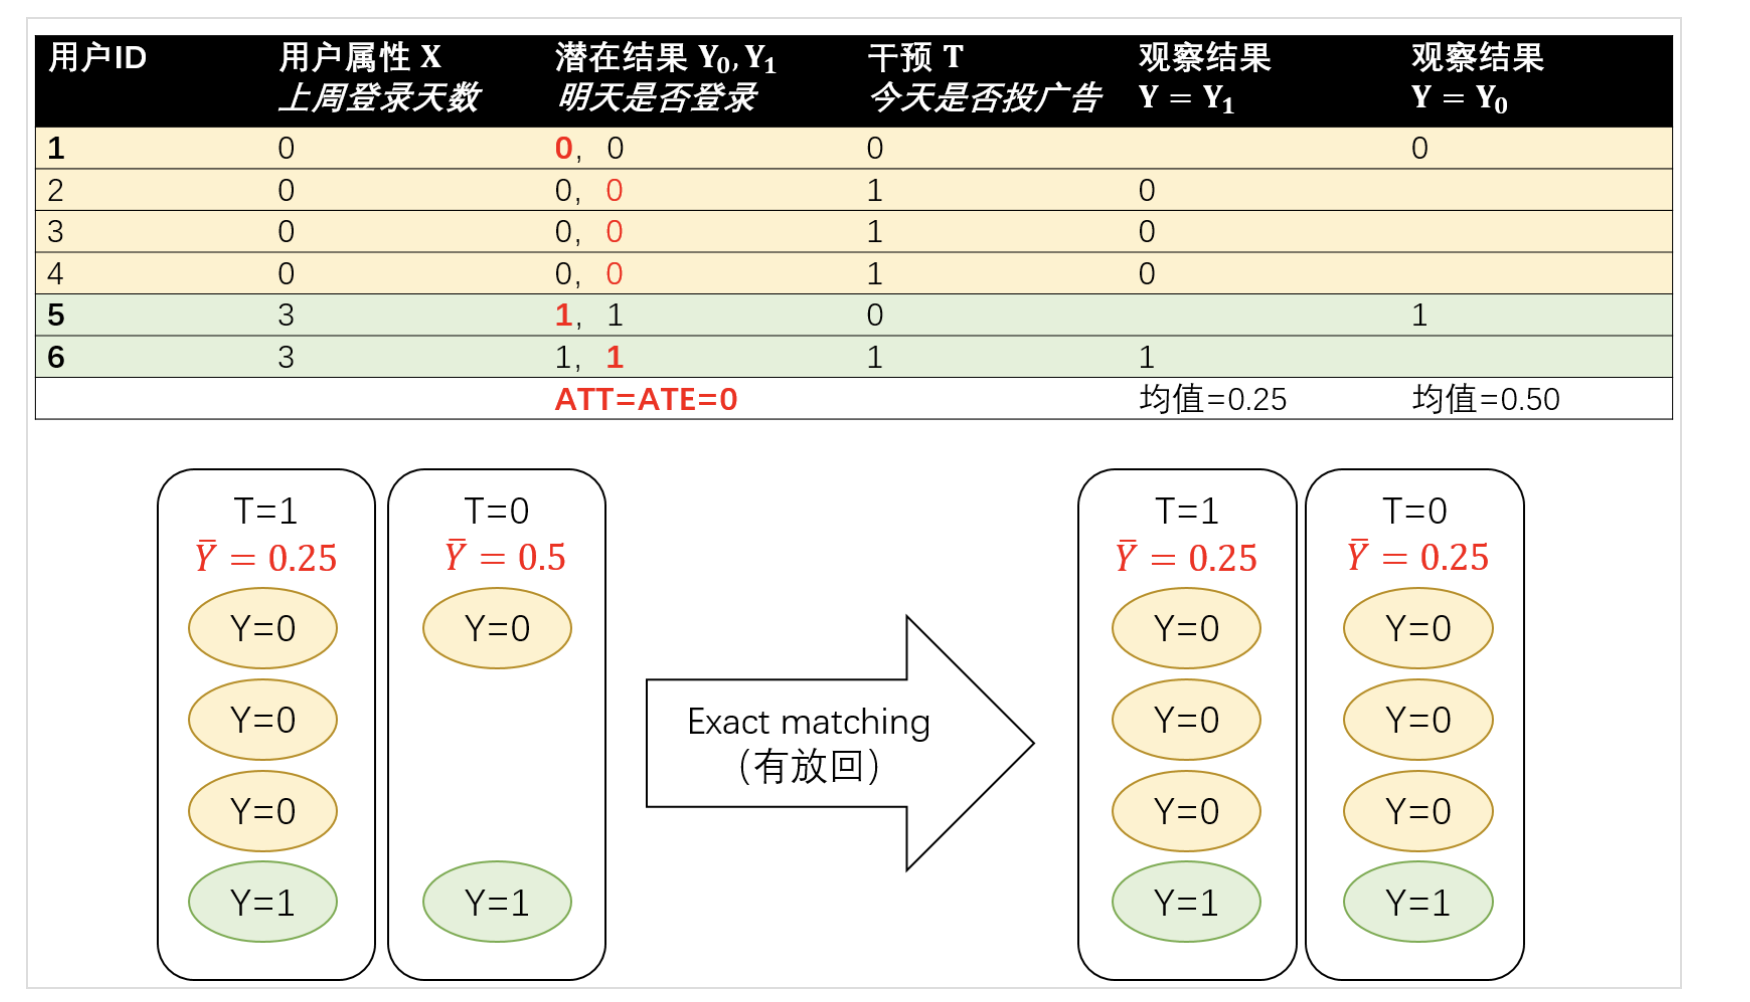
\includegraphics[width=1\textwidth]{fig/CasualInference-Game-Ad-2.png}
\end{figure}

Exact Matching 虽然直观,但是并不实用。“匹配用户的变量  $X$ 完全相等” 这个要求过于严格,随着变量 $X$ 的维度的增加,几乎不太可能有足量的匹配用户来下结论。

Exact Matching 的一个直观变种是 Distance Matching。我们可以对每一个 $T=1$ 的用户匹配一个距离最近并且不超过阈值的用户。这里 “距离” 如何定义、“阈值” 如何定义,也都需要更多的斟酌。另外,当我们通过距离来匹配时,其实是在潜意识里假设了变量 $X$ 的每一个维度都是同等 “重要” 的,这里也不一定科学。

为了科学有效地进行 Matching,一个经典的做法是 Propensity Score Matching,简称 PSM。在 PSM 方法中,我们首先对每一个用户计算一个倾向性得分(propensity score),定义为 $e(X)=Pr(T=1|X=x)$。接着我们根据倾向性得分将用户进行匹配 ,从而得到两个 $X$ 上看起来基本同质的用户组,然后统计得到 $ATT$。PSM 方法在实现上有许多值得深入介绍的地方,例如如何得到 “倾向性得分”、如何选择匹配方式(如一对一匹配、一对多匹配、分层匹配、有放回或无放回匹配)、如何衡量匹配质量等。关于更多 PSM 的细节,将会在下一篇文章里深入介绍。等不及的小伙伴也可以读一读参考资料([综述类 paper] Caliendo M, Kopeinig S. Some practical guidance for the implementation of propensity score matching[J]. Journal of economic surveys, 2008, 22(1): 31-72.)。

文献\cite{Causal_Inference_and_Stable_Learning}中有一个很好的Matching的例子:
\begin{figure}[H]
    \centering
    \caption*{对照组($T=0$)和实验组($T=1$),注意用户实际有不用的几类(绿色、深蓝色、浅蓝色)}
    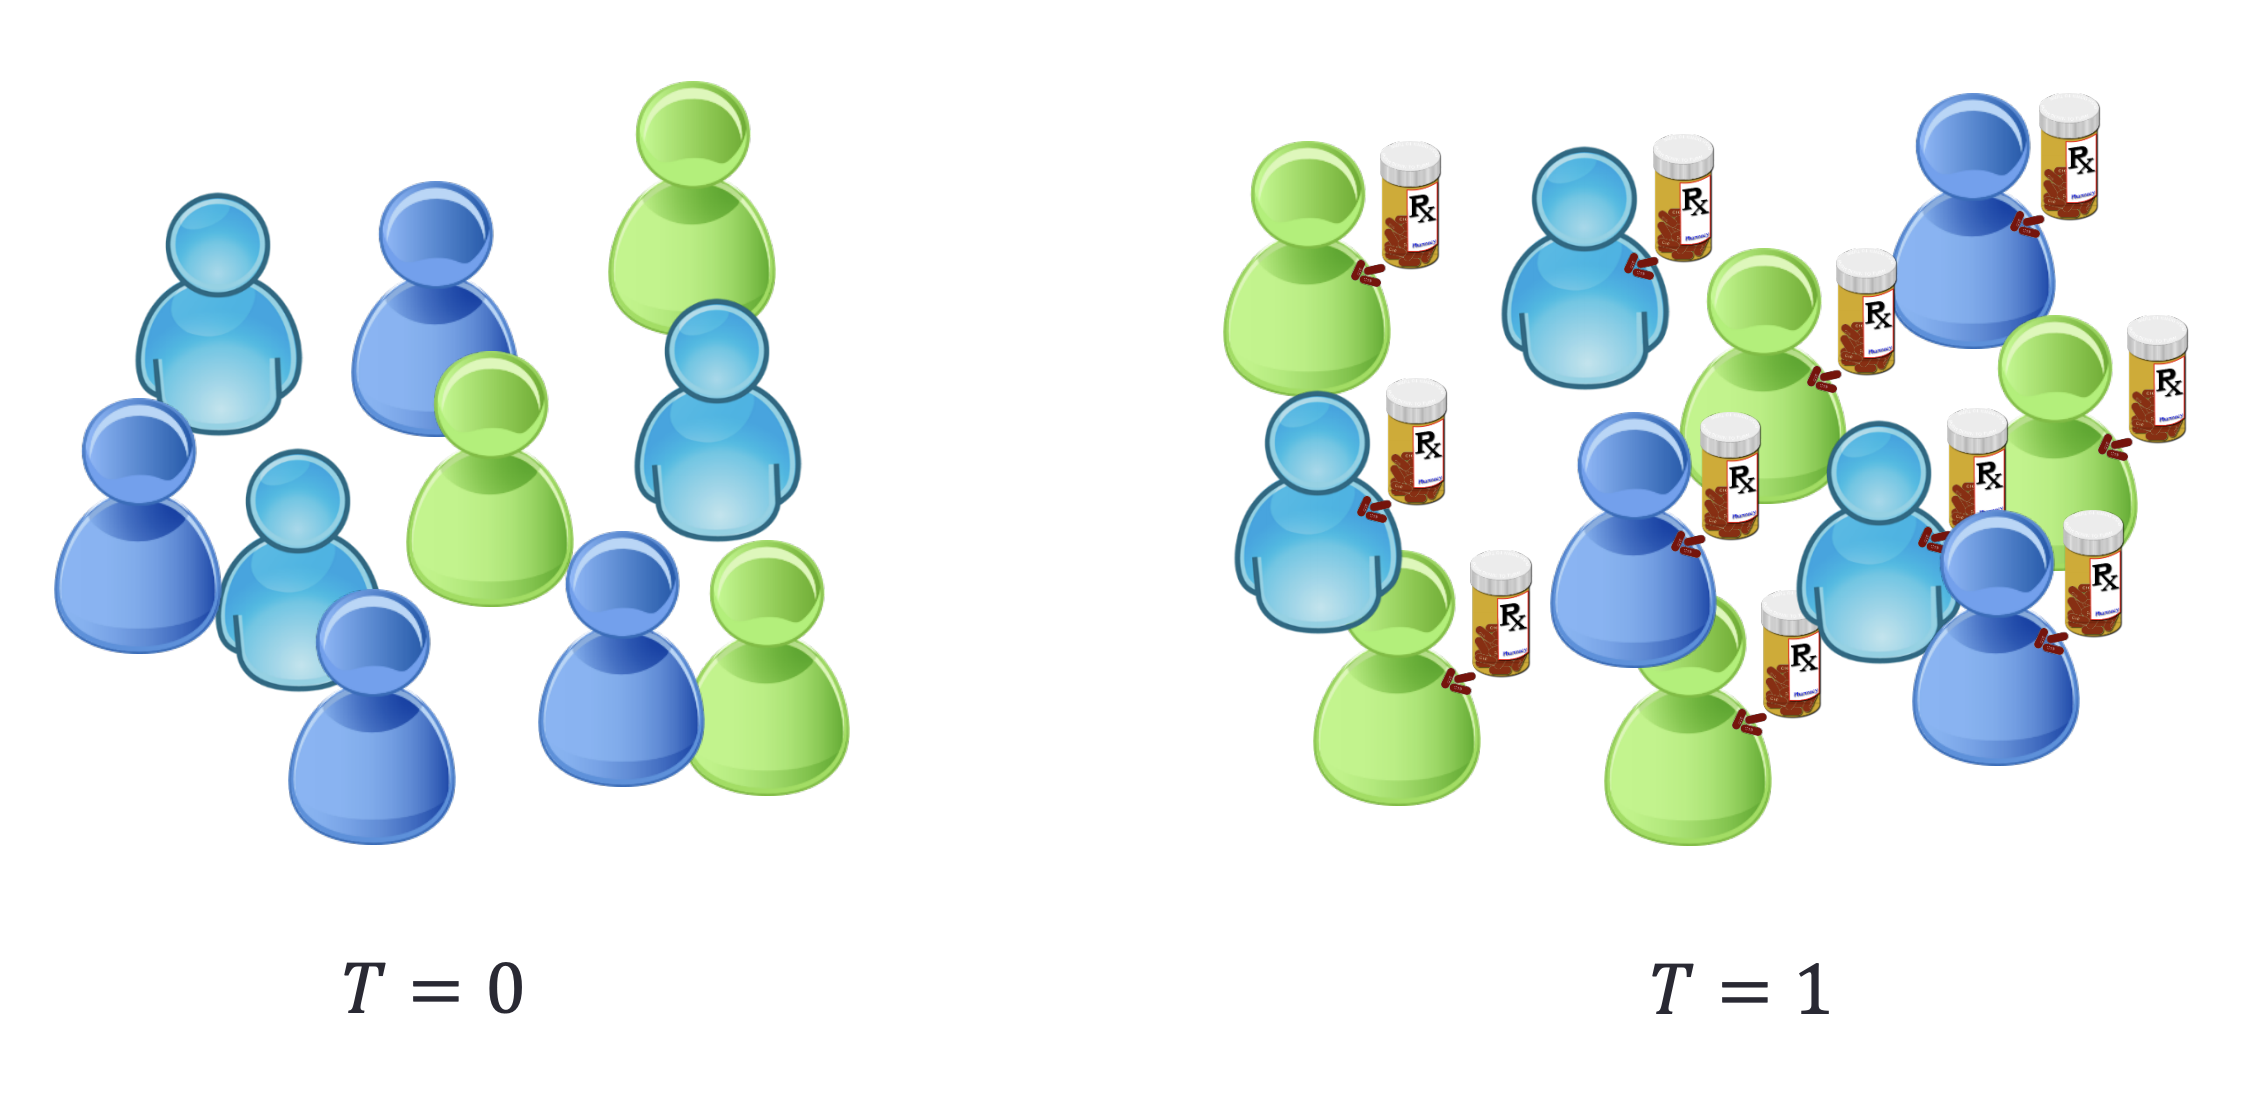
\includegraphics[width=0.8\textwidth]{fig/Causal_Inference_and_Stable_Learning-Matching-1.png}
\end{figure}

\begin{figure}[H]
    \centering
    \caption*{对用户进行 Matching,Matching 时的度量是:$Distance(X_i, X_j) \le \epsilon$;通过匹配,保证了同组的两个用户的其它特征都是基本相同的}
    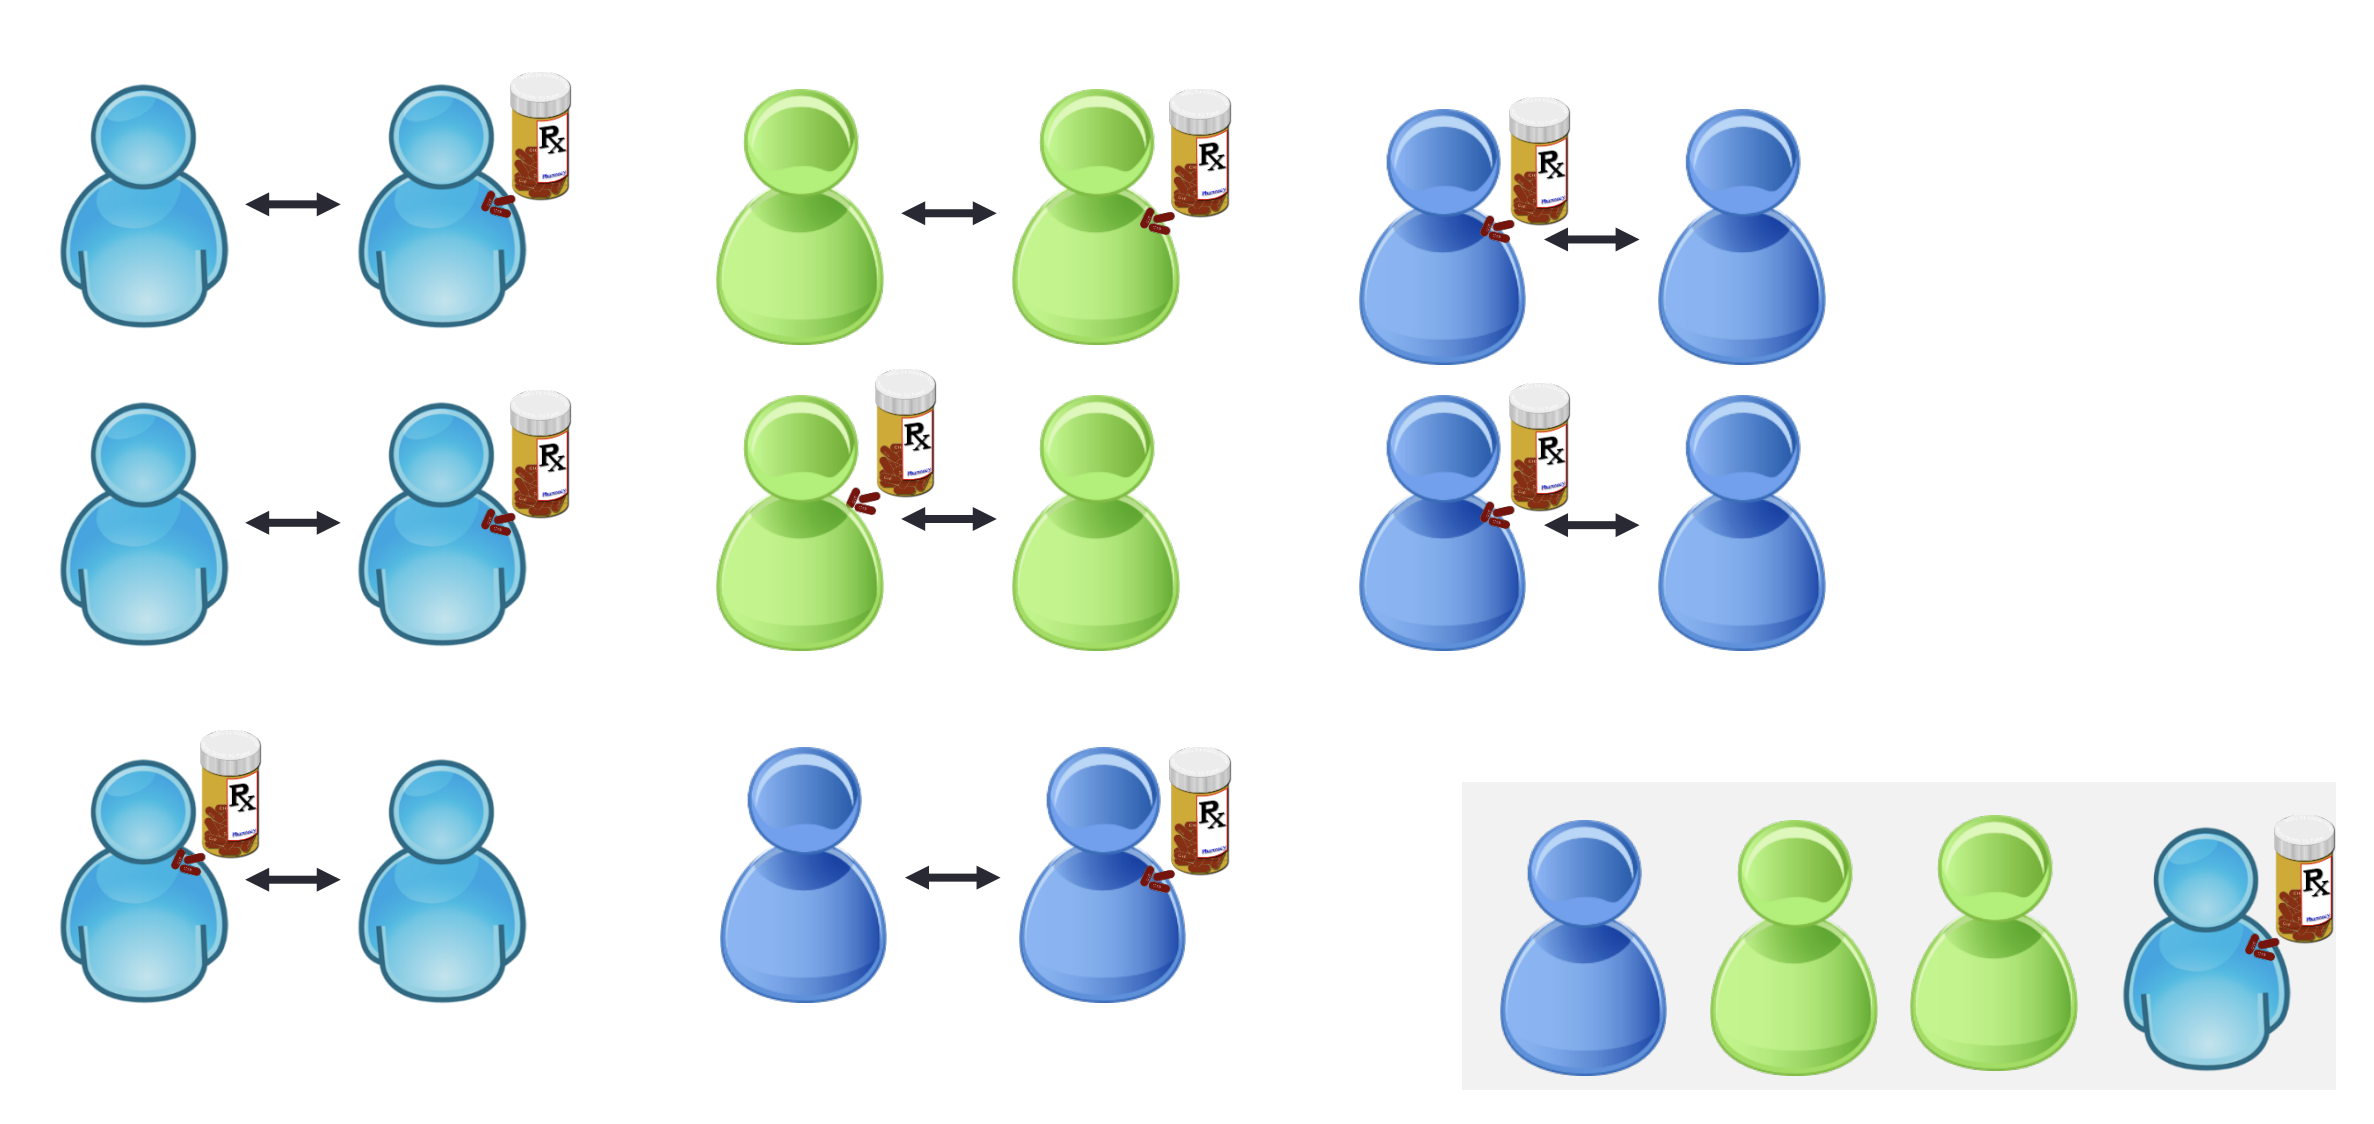
\includegraphics[width=0.8\textwidth]{fig/Causal_Inference_and_Stable_Learning-Matching-2.png}
\end{figure}

\subsection{Re-weighting方法}
目的是解决实验组和控制组分布不一致的问题。

方法是对采样数据赋予合适的权重,使得实验组和控制组的分布尽可能一致。

一些具体的 re-weighting 方法:略\cite{AAAI_2020_Tutorial_Representation_Learning_for_Causal_Inference}

\subsection{Stratification(subclassification/blocking)}
对原始数据进行分组,每个分组内,实验组和对照组尽可能保持一致;

Stratification adjusts the selection bias by splitting the entire group into subgroups, where within each subgroup, the treated group and the control group are similar under some measurements.

\subsection{Tree-based Methods}
Bayesian Additive Regression Trees (BART)

Classification And Regression Trees (CART)

\section{常见问题}
\subsection{因果推断(causal inference)是回归(regression)问题的一种特例吗?}
\url{https://www.zhihu.com/question/266812683/answer/895210894}

机器学习训练的模型已经无法写成简单的函数形式了,为什么因果推断还是以线性模型为主。因果推断可以表示成某种特殊的回归问题吗?把treatment variable $W$ 也当作一种binary feature,和其他的features $X$ 放在一起做回归,定义某种用$f(X, W)$预测$Y$的损失函数,treatment effect可以用$f(X, 1) - f(X, 0)$ 估计。这样做的问题在哪里呢?

我理解在observational study里需要处理数据(例如propensity score matching / re-weighting)使之尽可能满足unconfoundedness的假设,我的问题是:

1. 这种处理是否可以通过选取某种目标函数解上述回归问题自然导出?

2. 除此之外,因果推断和上述回归问题还有什么本质区别吗?

\subsubsection{引子:一个例子}
我们应该经常听说一个说法:因果关系并不是相关性,而回归分析只能研究相关性。这句话有一定的道理,却也不完全准确。真正要回答这个问题并不容易,所以我们先来举一个简单的例子。

假设你是一个品牌商,然后你对在城市 $c$ 广告的人均资金投入 $x_c$ 和实际的人均销售额 $y_c$ 之间的关系感兴趣。那么一个最简单粗暴的办法就是用看到的实际销售数据跑一个回归模型:
$$
y_c = bx_c + e_c
$$

其中 $e_c$ 是一个误差项, [公式] 就是我们关心的回归系数(假设我们已经把数据都中心化了,这样可以不考虑偏移项- $y_c$ 的“截距”)

当然跑回归需要数据:假设我们目前在两个城市有销售历史数据-北京和上海。。然后我们观察到在上海我们的人均广告投入是1元,人均销售额是10元;而在北京我们的人均广告投入是1角钱,人均销售额是1元。很显然,如果我们直接用这两组数据回归,我们便会得到:
$$
y_c = 10x_c
$$

\textbf{然而,这个式子似乎告诉了我们增加1元人均广告投入我们就能得到10元额外的人均销售额。这个理解真的对么?显然你肯定觉得有问题了,但关键的点在于,问题出在哪儿?}

\subsubsection{问题出在哪儿?}
在上述问题中,显然我们首先应该想到嗯我们的回归模型太简单了嘛,\textbf{肯定有其它很关键的因素(变量)没考虑到},所以就变成一个简单粗暴的二元关系式了。比如说,假设其实我们是卖咸粽子的,而上海人民普遍大多是咸粽子党,相比大多是甜粽子党的北京人民本来就对咸粽子的兴趣大得多。在这种情况下,这个对“咸粽子的兴趣程度”其实也会影响我们的销售额 $y_c$。另外,我们再假设我们的广告部门在做广告的时候本身也知道这点(这个是常识嘛),因此他们在广告投放的过程当中就是会在上海地区更卖力,而北京地区偷懒,因此这个对“咸粽子的兴趣程度”其实也会影响$x_c$

像这样\textbf{同时影响一个回归模型的 $y_c$ 和 $x_c$ 的变量(variable)我们就叫做confounding variable}。数学上来看,如果我们用 $(x,y,e)$ 代表 $(x_c,y_c,e_c)$的分布(数据量非常大的时候所趋近的统计规律),那么我们知道回归得到的系数 $b = \frac{Cov(x,y)}{Cov(x,x)}$(Cov表示协方差/Covariance)。利用 $y = bx + e$,我们可以把上式(右边)变形成
$$
b = \frac{Cov(x,bx + e)}{Cov(x,x) }= b + \frac{Cov(x,e)}{Cov(x,x)}
$$

也就是说,如果$Cov(x,e) = 0$ ,我们这个回归跑出来的 $b$ 就是无偏的,能反应数据背后的统计规律,反之就不行了。

注意这里有个值得澄清的点:如果我们只是希望用回归模型去做预测(prediction),那么实际上前一节的二元回归可能也就行了。但是这往往不是我们的主要目的,事实上就跟前一节考虑的问题那样,我们想知道的是增加一些广告投入,对销售额的影响(变化)是怎样的。\textbf{即某些回归模型的变量 $x_c$改变对 结果$y_c$的影响}。

因此,我们\textbf{并不应该简单地把这里的问题看成“回归模型里缺了某些变量”}。事实上,对任何实际使用的回归模型,你都可以说它缺了某些变量。这里的问题实实在在的是,\textbf{存在一个我们没有考虑的变量,同时影响着我们粽子的销售额 $y_c$ 和投入成本  $x_c$ }。而在我们简单的二元回归模型里,因为我们没有考虑这个confounding variable(因此它隐含在 $e$ 里),使得 $x_c$ 和  $y_c$ 也会变得有相关性。在我们的粽子例子中,因为对咸粽子兴趣更大的城市会自然让该城市的广告投入和销售额增加,也就是说仅对 $y_c$和 $x_c$ 做回归会过高估计$x_c$变化对 $y_c$的影响。

这便是因果推断的起点:\textbf{如何通过已有的数据更准确的推断各种变量之间的因果关系(某些变量变化对结果的影响)}?

接下来我们就讨论一些可能有用的方法。

\subsubsection{Difference in Differences(DiD)}
当然目前为止我们还没有回答题主的问题。把DiD放在前面因为这个和题主的利用f(X,1)-f(X,0)估计treatment effect想法相似(这在实际中也是很powerful的一种想法)。当然要用DiD,一般我们需要所谓的纵向(longitudinal)数据, 即在一条时间线上不同点上的数据。

比如在我们的例子里,我们在两个城市一开始都有一段时间没有任何广告投入( $x_c = 0$),然后比如3月我们在上海投放了一波广告(北京没有),4月我们在北京投放了一波广告(上海没有)。我们其实就可以把这个有没有投放广告看成是一种treatment,而在这样的数据情况下我们就可以来估计我们想要的因果关系。具体来说,我们考虑一段相似的时间段,如果这段时间段里没有投放广告,那么这段时间的销售额可以看成是“对照组”(control group)的数据,反之就是“投放组”(treated group)。我们记

$s_{TA}$时间段结束后投放组的销售额

$s_{TB}$ 时间段开始前投放组的销售额

$s_{CA}$时间段结束后对照组的销售额

$s_{CB}$时间段开始前对照组的销售额

那么我们确实可以将treatment effect(投放广告对销售额的作用)估计为:

$$
(s_{TA} - s_{TB}) - (s_{CA} - s_{CB})
$$

即“差的差”DiD。当然这个式子看起来也是无比简单,而这个treatment effect实际就如题主所说的,完全可以用回归来估计(估计的时候甚至还可以加上更多的变量,比如季节影响啊天气啊等等),也可以像@慧航所说的用别的非参方法如bootstrap,或者神经网络:这些估计方法都只是“工具”,而不是模型。

注意实际上这里我们估计的是投放组\textbf{真实的结果(投放广告之后的销售额)} $s_{TA}$ 和投放组的\textbf{反事实(counterfactual,即投放组如果没有投放广告在时间段结束后的销售额的差)} $s_{TF}$。并且还依赖了这样一个假设,即\textbf{根据反事实,如果投放组其实没有投放广告,那么这个时间段投放组的销售额变化和对照组应当是一样的}(数据采集的人们的行为是同质的-homogeneous):
$$
(s_{TF} - s_{TB}) = (s_{CA} - s_{CB})
$$

\subsubsection{控制实验(Controlled Experiments)和自然实验(Natural Experiments)}
为了研究因果关系,如果有条件做“实验”显然是最直接的办法。当然实验大体也分为两种类型,一种是我们可以控制各种变量,另外一种就是其实并不能(比如很多医疗手术/用药的数据-人为想“控制”出一些“对照组”显然是不道德的)。

就拿我们的问题来说,实际上广告投放是我们完全可以控制的。相比前面的DiD,我们完全可以做的更好:我们完全可以在同样的月份,不同的城市里,根据顾客的资料信息将他们分成大致类似的两组,然后一组对他们进行广告投放一组完全不进行(对照和投放组),然后观察这个月份这两组消费者销售额的变化情况。

当然如果这并不现实,那么其实就如@刘垚 所说的随机性(randomization)的重要性就更大了(随机性对估计treatment effect其实一直都很重要)。也就是说即使我们无法完美的有控制组和对照组的数据,是否可以自然观察到针对是否有treatment比较随机的结果(比如我们的广告投放是在固定的商场门口,然后来访问商场的顾客分布相当的随机无规律),以减小估计的误差。

\subsubsection{工具变量(Instrumental Variable)}
这也是计量经济学里非常常用的技巧。还记得前面卖粽子例子里我们说二元回归关系一个主要的问题是 $e_c$ 其实同时跟 $y_c, x_c$有相关性么?然而,如果我们可以找到一个\textbf{工具变量,只通过变量 $x_c$ 来影响结果 $y_c$,那么我们就其实可以用这个工具变量作为“仪器”来“沿着” $x_c$ 独立于 $e_c$ 运动地“测量”$y_c$ 的变化}(我的理解,这句话有点按照特征向量进行分解的意思)。

如果我们把这个工具变量叫做 $z_c$。在我们的卖粽子例子里,数学上就有
$$
y_c = bx_c + e_c
$$
$$
x_c = az_c + d_c
$$

我们其实就有了两个回归模型。而我们注意到这两个回归模型结合在一起就给了我们:
\begin{align*}
b^{iv} &= \frac{Cov(z,y)}{Cov(z,x)} \\
         &= \frac{Cov(z,bx+e)}{Cov(z,x)} \\
         &= \frac{bCov(z,x) + Cov(z,e)}{Cov(z,x)}\\
         & = b
\end{align*}

\textbf{这是一个对$b$的无偏估计}!而本质上我们就是利用了工具变量的特性将 $e_c$ 对$x_c, y_c$的复杂影响给排除掉了(因为工具变量跟 $e_c$是独立的)。而这种利用工具变量的回归分析有时也被称之为\textbf{两阶段回归}(two-stage regression; 留给大家思考: $b^{iv}$的估计其实也可以看成是先做了一步回归,然后利用上一步回归的结果带入下一步回归中-那么这里具体是哪两步回归呢?)

当然,因果推断的招式很多,这里我只是浅尝辄止地谈了谈计量经济里用的比较多的几个方法,其它的像Regression Discontinuity之类的在某些场合也很有用(比如历史数据只有几个 $x_c$ 和相应的 $y_c$)。像Judea Peral几乎一己之力创造的基于贝叶斯网络和图模型的招式([2]),就完全落在另一个流派里了。我觉得,对因果关系的研究,从过去,到现在,直到将来都将一直会是人类科学研究的重点之一:比如说,究竟有哪些重要的因素,在何种影响和条件下,会促发某些癌症?反过来说,又有哪些关键的因素,条件,treatment,可以逆转癌症的扩散和恶化?时至今日,回归分析仍然是所有人类研究里最最常见的工具(也仍是目前因果推断研究的主流方法),而它伴随着现在的人工智能\&机器学习热潮,又能带领我们在因果性的推断旅程里前进到何方呢?






%\printbibliography
\bibliography{../ref}
\bibliographystyle{IEEEtran}
\end{document}